\documentclass[a4paper,12pt]{article}

% > Page setup
\usepackage[left=2.25cm, right=2.25cm, top=2.5cm, bottom=2.5cm]{geometry}
\usepackage{setspace}       		% line spacing
\usepackage{graphicx}       		% image support
\graphicspath{{resources/}} 		% image folder
\doublespacing              		% double spacing
\renewcommand{\arraystretch}{0.6}	% since the forced double spacing ruins everything
\pagenumbering{arabic}      		% page numbering

% > Math packages
\usepackage{physics}							% well, it's a physics package but whatever
\usepackage{amsmath, amssymb, amsfonts, amsthm} % math symbols & environments

% > References & bibliography
\usepackage{cite}                                  % BibTeX citation support
\usepackage[notlof,nottoc,numbib]{tocbibind}       % include bibliography in ToC

% > Styling & utilities
\usepackage{xcolor} % colored text

% > Custom commands

% fix ugly Nabla physics package operators
\renewcommand\gradient[1]{\nabla#1}
\renewcommand\divergence[1]{\nabla\vdot#1}
\renewcommand\curl[1]{\nabla\cp#1}

% Vectors and symbols
\newcommand{\ihat}{\hat{\imath}}
\newcommand{\jhat}{\hat{\jmath}}
\newcommand{\rhat}{\hat{r}}
\newcommand{\nhat}{\hat{n}}
\newcommand{\thetahat}{\hat{\theta}}
\newcommand{\fatf}{\mathbf{F}}         		% vector field F
\newcommand{\fatomega}{\boldsymbol{\omega}} % vorticity
\renewcommand{\theta}{\vartheta}      		% use vartheta for theta

% Derivatives
\newcommand{\der}[2]{\frac{\mathrm{d} #1}{\mathrm{d} #2}}           % total derivative
\newcommand{\partialder}[2]{\frac{\partial #1}{\partial #2}}        % partial derivative
\newcommand{\materialder}[2]{\frac{\mathrm{D} #1}{\mathrm{D} #2}}   % material derivative

% Miscellaneous
\newcommand{\justify}[1]{\text{\color{gray}(#1)}} 								% inline justification notes
\newcommand{\definedas}{\stackrel{\Delta}{=}}     								% "defined as" symbol
\newcommand{\referto}[1]{\textsuperscript{\color{darkgray}\tiny[see \ref{#1}]}}	% citation command
\newcommand{\needcitation}{\textsuperscript{\normalfont[Citation needed]}}		% temporarily mark where I need to cite
\renewcommand{\qedsymbol}{\hfill\ensuremath{\blacksquare}}						% make the QED symbol great again
\newcommand{\vecpadding}{\vspace*{0.15cm}}										% for when fractions et cetera get too close in a vector

% Research question
\newcommand{\researchquestion}
{
	How can vector calculus be applied to model and analyze 
	incompressible fluid flow in two-dimensional spaces with 
	circular obstacles, and what mathematical insights
	does this provide about real-world fluid systems?
}

% > Theorems
\newtheorem{theorem}{Theorem}[section]
\newtheorem{corollary}{Corollary}[theorem]
\newtheorem{lemma}[theorem]{Lemma}

% > Document

\begin{document}

% > Title page
\begin{titlepage}
	\begin{center}
		\vspace*{2cm}
		\Large On the modelling of steady, inviscid and incompressible fluid flow around a two-dimensional cylinder

		\vspace{1.5cm}
		\normalsize Research question: "\textbf{\researchquestion}"

		\vspace{1.5cm}
		\large\textbf{Mathematics AA HL}

		\vfill
		\color{darkgray} Word Count: 3419
	\end{center}
\end{titlepage}

% > Table of contents
\tableofcontents\newpage
\section{Introduction}
Fluid dynamics is today a cornerstone to several fields of study, including ærospace engineering and meteorology.
Real world fluid behaviour is intricate and complex. Therefore, to gain insights into the governing principles of
fluid flow, simplified and idealised models are used. This essay investigates the application of vector calculus
to model and analyse steady, inviscid, and incompressible fluid flow in two-dimensional spaces around a circular
obstacle. These idealisations allow for the derivation of some of fluid dynamic's key mathematical formulæ and
provides a foundation for understanding less idealised fluids.

This essay will address the question: "\researchquestion" Through the derivation of the velocity potential and
vector field, this essay aims to demonstrate how fundamental laws of fluid motion can be expressed and used through
vector calculus.

% Aim & scope
\subsection{Aim \& scope}
The scope of this essay will be limited to the theoretical modelling of fluid flow in a two-dimensional space
as a vector field under idealised conditions forming steady, inviscid and incompressible fluid flow through the 
derivation of the velocity-potential. The analysis will be centred on the application of vector calculus to derive
fundamental formulæ and describe fluid behaviour around a stationary circular obstacle. Consequently, this essay
will not touch on viscous effects, turbulent flow or three-dimensional analysis, nor will it involve any experimental 
validation. The focus is on the mathematical derivation and analysis of the idealised model.

% Background
\subsection{Background}
\subsubsection{Glossary}
\begin{defn} % steady flow
    \definedterm{Steady flow} refers to flow in which the velocity at every point does not change over time \cite{CRACIUNOIU2001559}.
\end{defn}
\begin{defn} % inviscid flow
    \definedterm{Inviscid flow} is the flow of a fluid with 0 viscosity \cite{ANDERSON20031}.
\end{defn}
\begin{defn} % incompressible fluid
    An \definedterm{incompressible fluid} is a fluid whose density at every point does not change over time \cite{AHMED2019331}.
\end{defn}
\begin{defn} % scalar field
	A \definedterm{scalar field} is a function mapping points in space to scalar quantities such as temperatures.

	\begin{figure*}[!ht]
		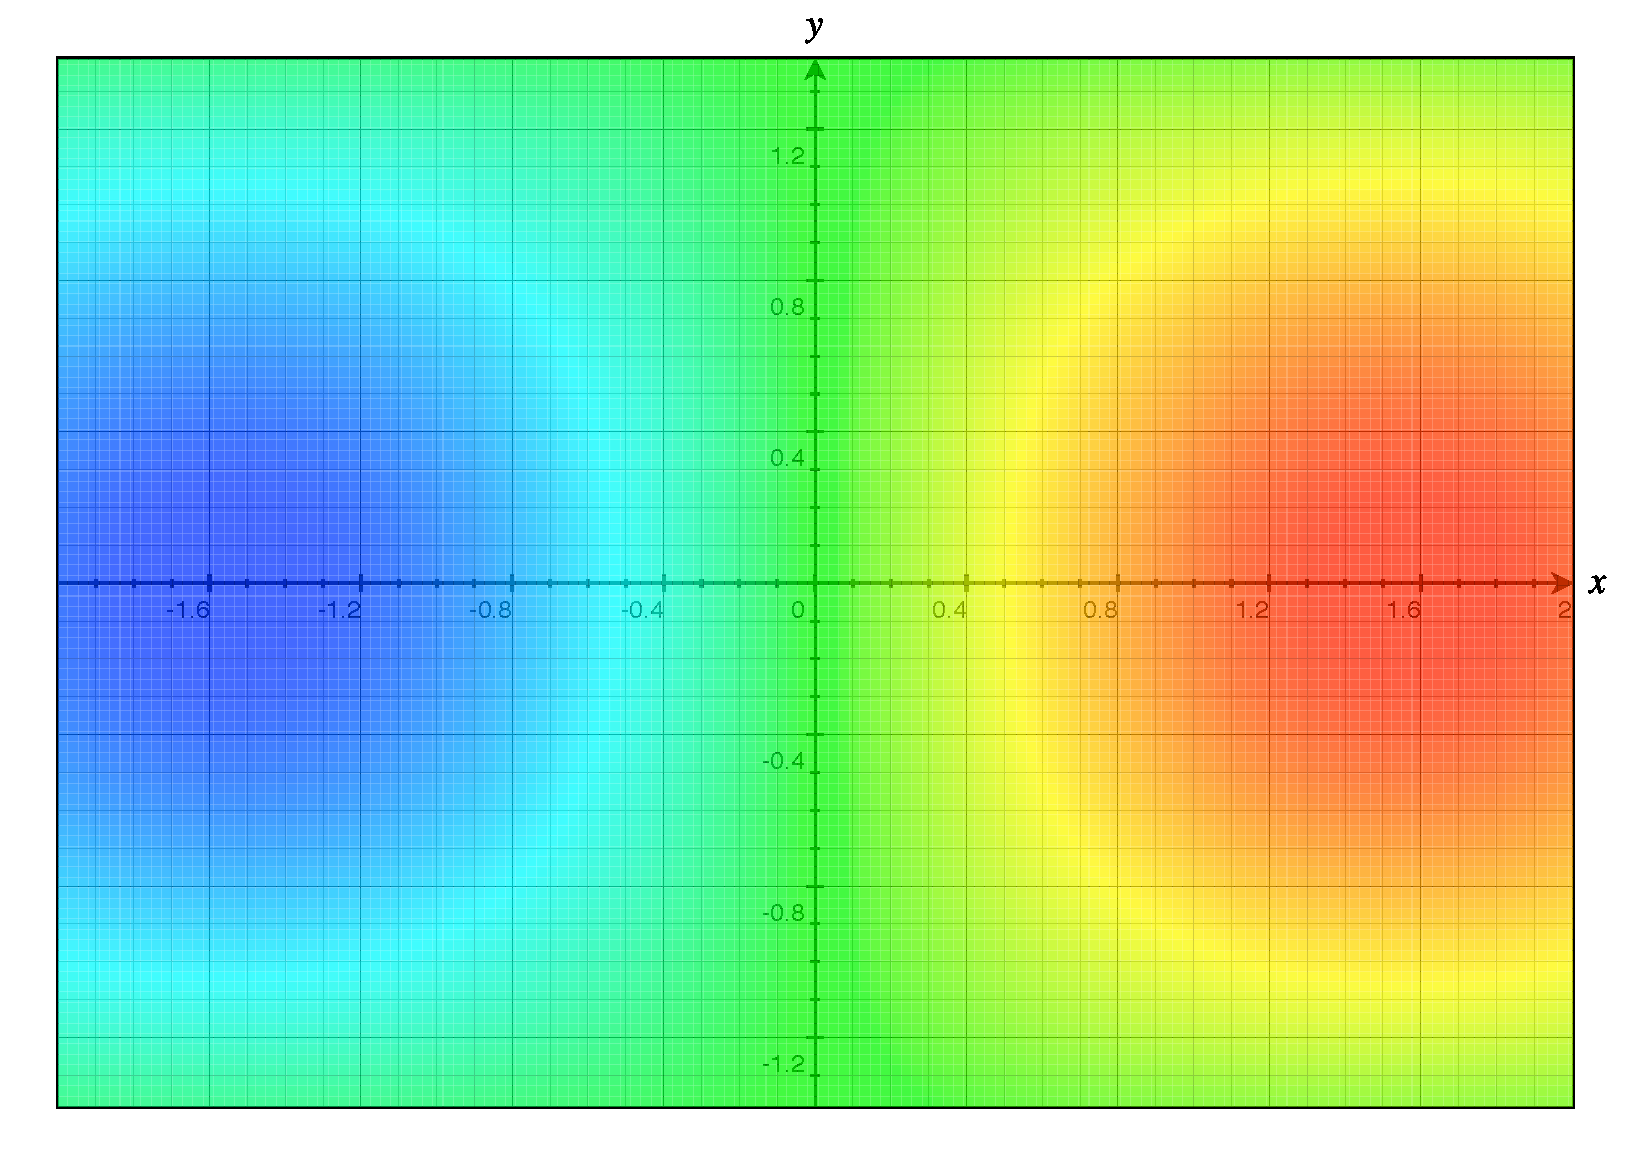
\includegraphics[scale=0.5]{scalar_field_example.pdf}
		\centering
		\caption{Scalar field plotted for the function $f(x,y)=\sin(x)\cos y$}
	\end{figure*}
\end{defn}
\begin{defn} % vector field
    A \definedterm{vector field} is a function mapping points in space to vector quantities \cite{BREZINSKI20063}. In
	the case of fluid dynamics, vector fields often model quantities like fluid velocity.

	\begin{figure*}[!ht]
		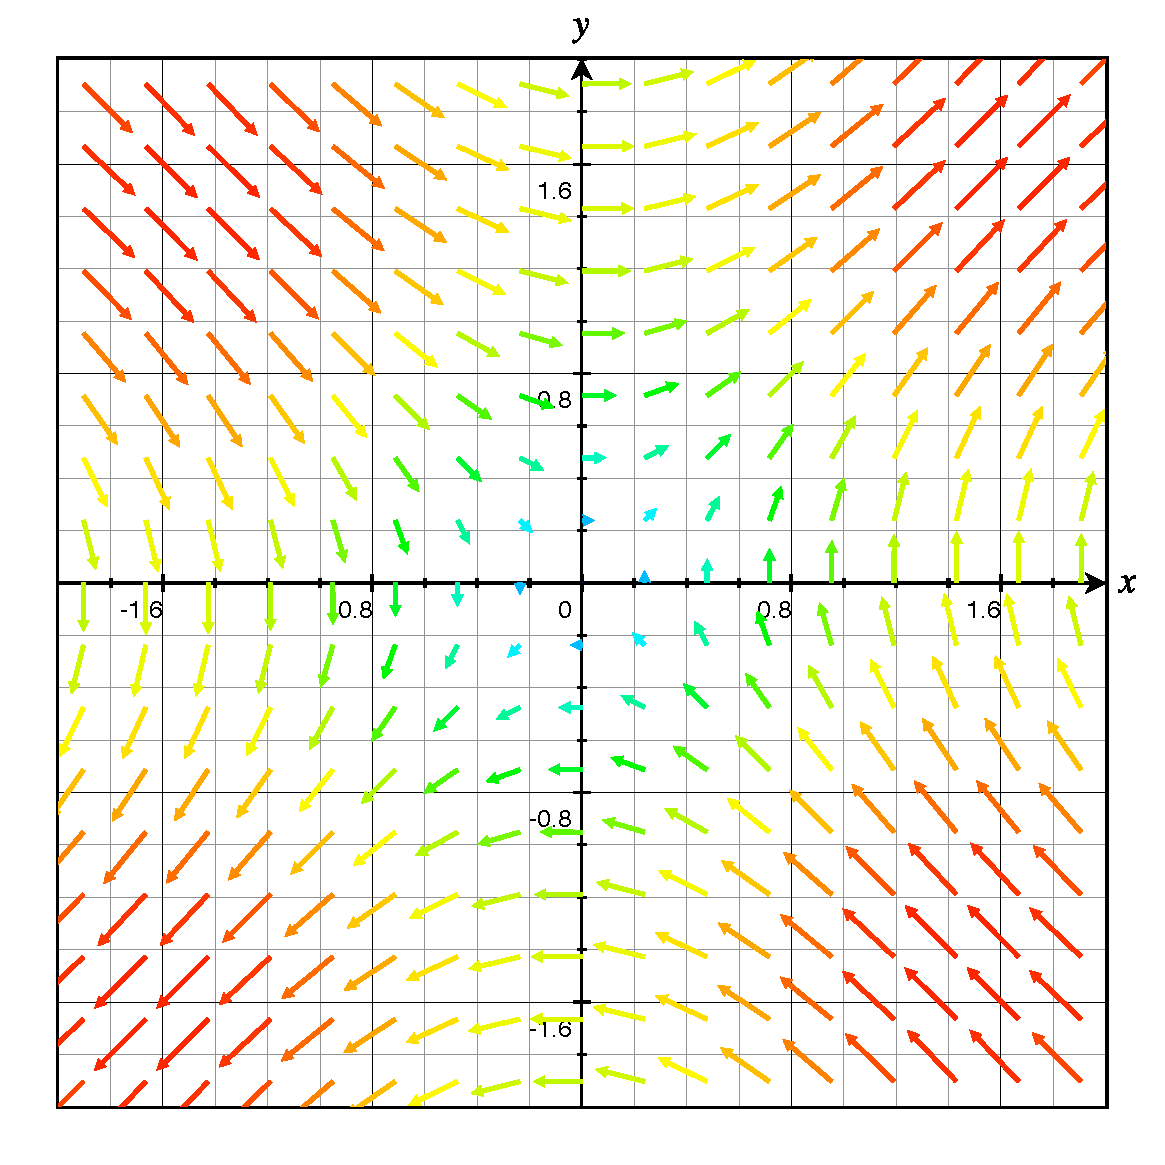
\includegraphics[scale=0.5]{vector_field_example.pdf}
		\centering
		\caption{Vector field plotted for the function $f(x,y)=\begin{pmatrix}
			\sin y\\\sin x
		\end{pmatrix}$}
	\end{figure*}
\end{defn}
\begin{defn} % velocity potential
	The \definedterm{velocity potential} $\phi$ is a scalar field whose gradient is the velocity vector field of some
	fluid, mathematically $\mathbf{V}=\nabla\phi$. The quantity is defined for irrotational flow which is a resulting
	property of the idealisations made in this essay\referto{theorem:kelvin}.
\end{defn}

\subsubsection{Notation}
Vector calculus, like one-variable calculus, has no standardized notation. This essay will employ the following
notation:
\begin{itemize}
	\item $\nabla$:
	\begin{itemize}
		\item $\gradient{F}$: The gradient of some scalar field $F$.
		\item $\divergence{\fatf}$: The divergence of some vector field $\fatf$.
		\item $\curl{\fatf}$: The curl of some vector field $\fatf$.
		\item $\nabla_\vec{v}f$: The directional derivative of $f$ in the direction of some vector $\vec{v}$
	\end{itemize}
	\item $\Delta$: The Laplacian operator
	\item $\disk{x}{y}$: The set of the points in an open disk centred at $\point{x}{y}$ with radius $\delta$
	\item $\ihat\,\&\,\jhat$: Unit vectors in the positive $x$ and $y$ directions respectively.
	\item $\rhat\,\&\,\thetahat$: Unit vectors in the positive $r$ and $\theta$ directions respectively.
\end{itemize}

\subsubsection{The mean value theorem}\label{section:MVT}
[REPHRASE LATER] The mean value theorem, along with other lemmas introduced in section \ref{section:MVT} are important in the proving of other theorems.
\begin{lemma}[The extreme value theorem]\label{lemma:MINMAX}
	If a function $f$ is continuous on the finite interval $[a,b]$, then there exists $A,B\in[a,b]\ni f(A)\leq f(x)\leq f(B)\,\forall x\in[a,b]$.
	Thus, at the points $A$ and $B$, $f$ has an absolute minimum $m=f(A)$ and an absolute maximum $M=f(B)$.
\end{lemma}
\begin{lemma}[Rolle's theorem]\label{lemma:ROLLES}
	If a function $f$ is continuous on the interval $[a,b]$ and differentiable on $(a,b)$, and $f(a)=f(b)$, then $\exists\,c\in(a,b)\ni f'(c)=0$.
	\begin{proof}
		Consider two cases:
		
		\textbf{Case 1: $f$ remains constant over $[a,b]$}\newline
		If $f(x)=f(a)=f(b)\,\forall x\in(a,b)$, then $f'(x)=0$, and the theorem holds trivially. 
		
		\textbf{Case 2: $f$ is not constant over $[a,b]$}\newline
		If $f$ is not constant over $[a,b]$ and $f(a)=f(b)$, then \lemmaref{lemma:MINMAX} asserts that there must exist an absolute maximum
		or minimum that occur at some point $\eta\in(a,b)$. Since $f$ is differentiable over $(a,b)$, then any point $\eta$ where an absolute
		extremum occurs must also be a local extremum. Consider the case where $\eta$ is a local maxima (the proof for the case of local minima
		is analogous). Then let the interval $I=(\eta-\delta,\eta+\delta)$ for some $\delta>0\ni\forall X\in I,f(X)\leq f(\eta)$.

		Let $h<0$ be a number sufficiently small such that $\eta+h\in I$. $f(\eta+h)\leq f(\eta)\implies f(\eta+h)-f(\eta)\leq0$. Thus,
		$$
			\frac{f(\eta+h)-f(\eta)}{h}\geq0\because\left\{\begin{matrix}
				f(\eta+h)-f(\eta)&\leq0\\
				h&\leq0
			\end{matrix}\right.
		$$
		Taking the left-hand limit as $h\rightarrow0$,
		$$
			\lim_{h\rightarrow0^-}\frac{f(\eta+h)-f(\eta)}{h}=f'(\eta)
		$$
		Now let $H>0$ be a number sufficiently small such that $\eta-H\in I$.
		\begin{align*}
			\frac{f(\eta+H)-f(\eta)}{H}&\leq0\because\left\{\begin{matrix}
				f(\eta+H)-f(\eta)&\leq0\\
				H&\geq0
			\end{matrix}\right.\\
			\lim_{H\rightarrow0^+}\frac{f(\eta+H)-f(\eta)}{H}&=f'(\eta)
		\end{align*}
		Thus,
		\begin{align*}
			0\geq\lim_{H\rightarrow0^+}\frac{f(\eta+H)-f(\eta)}{H}=&f'(\eta)=\lim_{h\rightarrow0^-}\frac{f(\eta+h)-f(\eta)}{h}\geq0\\
			\therefore\,&f'(\eta)=0
		\end{align*}
		Since the same would apply for local minima, then for any local extrema $\eta\in(a,b)$, of which \lemmaref{lemma:MINMAX} asserts
		there must exist at least one, $f'(\eta)=0$.
	\end{proof}
\end{lemma}
\begin{lemma}[The mean value theorem]\label{lemma:MVT}
	For any function $f$ continuous on the interval $[a,b]$ and differentiable on the interval $(a,b)$,
	$\exists\,c\in(a,b)\ni$
	\begin{equation}\label{equation:MVT}
		f'(c)=\frac{f(b)-f(a)}{b-a}
	\end{equation}
	\begin{proof}
		Consider the region of some function $f$ on the finite interval $[a,b]$ over which $f$ is continuous and differentiable over $(a,b)$.
		Let the function $L$ represent the straight line between the points $\point{a}{f(a)}$ and $\point{a}{f(b)}$, given by the expression:
		$$
			L(x)=f(a)+\frac{f(b)-f(a)}{b-a}(x-a)
		$$
		Now consider the function $g$, defined as the difference between $f$ and $L$:
		$$
			g(x)=L(x)-f(x)=f(a)+\frac{f(b)-f(a)}{b-a}(x-a)-f(x)
		$$
		\begin{center}			
			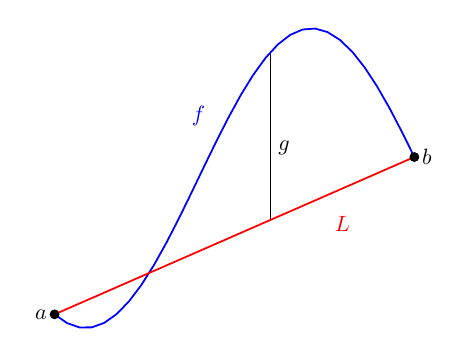
\begin{tikzpicture}[scale=0.8]
				\begin{axis}
				[
					hide axis,
					domain=-4:4
				]
				\draw[color=black, thick] (1, -0.2790) -- (1, 0.8415);
				\addplot[samples=30, color=blue, thick, domain=-2:3] { sin(deg(x)) };
				\addplot[samples=2, color=red, thick, domain=-2:3] { sin(deg(-2))+(sin(deg(3))-sin(deg(-2)))/5*(x+2) };
				\node[color=black, anchor=west] at (1, 0.2) { $g$ };
				\node[color=blue, anchor=south] at (0, 0.3) { $f$ };
				\node[color=red, anchor=north] at (2, -0.2) { $L$ };
				\filldraw[black] (3, 0.1411) circle (2pt) node[anchor=west] {$b$};
				\filldraw[black] (-2, -0.9093) circle (2pt) node[anchor=east] {$a$};
				\end{axis}
			\end{tikzpicture}
		\end{center}
		Computing the derivative of $g$ with respect to $x$ gives:
		$$
			g'(x)=\frac{f(b)-f(a)}{b-a}-f'(x)
		$$
		Since $g(a)=g(b)=0$, \lemmaref{lemma:ROLLES} asserts that there is at least one point $c\in(a,b)$ such that $g'(c)=0.$ Thus, at $c$,
		\begin{align*}
			0=g'(c)&=\frac{f(b)-f(a)}{b-a}-f'(c)\\
			\implies f'(c)&=\frac{f(b)-f(a)}{b-a}
		\end{align*}
	\end{proof}
\end{lemma}

% \begin{tikzpicture}
% \begin{axis}[
% title={$x \exp(-x^2-y^2)$},
% domain=-2:2,
% view={0}{90},
% colormap/viridis,
% colorbar,
% ]
% \addplot3[
%     surf,
% 	shader=interp,
% 	samples=20
% ]
% { sin(deg(x))*cos(deg(y)) };
% \end{axis}
% \end{tikzpicture}
\section{Mathematical background}
\subsection{The fundementals of vector calculus}
One dimensional calculus provides the tools for finding the slope of some function $f$ with respect to some variable $x$ at some point through the derivative, often denoted by Leibniz's notation $\der{f}{x}$, representing the ratio between some small change in $f$ after some small change in $x$. For example, the equation of the slope of the function $f(x)=x^2$ at some point can be calculated using the formal definition of a deriative:
\begin{equation}
	\der{f}{x}=\underbrace{\lim_{h\rightarrow0}\frac{f(x+h)-f(x)}{h}}_\text{\hidewidth The formal definition of a derivative\hidewidth}\\
\end{equation}
\begin{align*}
	f(x)=x^2\rightarrow\der{f}{x}&=\lim_{h\rightarrow0}\frac{(x+h)^2-(x)^2}{h}\\
	&=\lim_{h\rightarrow0}\frac{x^2+2xh+h^2-x^2}{h}\\
	&=\lim_{h\rightarrow0}\frac{2xh+h^2}{h}\\
	&=\lim_{h\rightarrow0}2x+h=2x
\end{align*}
More conveniently, Lagrange's or Euler's notation for the derivative is often used to avoid excessive writing.
$$\der{f}{x}\equiv f'(x)\equiv \mathrm{D}f$$
For the purposes of this essay, the formal definition of a derivative will not be used to calculate each derivation, rather common patterns and rules (such as the power rule, product rule, etc.) will be used. 

Multi-variable calculus introduces the partial derivative, which functions the same as a normal derivative but treats all variables except for the one being differentiated by as constants, allowing for the derivation of multi-variable functions.
\begin{align*}
	f(x,y)=x^2+y^2\implies\partialder{f}{x}=2x && \justify{power rule}
\end{align*}
However, the partial derivative only provides part of the picture, since it only takes into consideration one variable. Defining one single full picture "derivative" of a multi-variable function is not possible, since there are an infinite number of "slopes" at some point, and what you want the derivative to achieve will depend on your goal (e.g. what direction you want to differentiate in).

\subsubsection*{The nabla operator}
The nabla operator, denoted $\nabla$ (pronounced nabla or del), is a vector filled with partial derivatives with respect to each variable some function $f$ takes. For example, consider some function $f:\mathbb{R}^n\rightarrow\mathbb{R}^m$, nabla would then be defined as:
\begin{equation}
	\left.\nabla=
	\begin{bmatrix}
		\partialder{}{x} \\
		\partialder{}{y} \\
		\partialder{}{z} \\ 
		\vdots 	         \\
	\end{bmatrix}
	\color{gray}\right\} \color{gray}n\text{ times}\color{black}
\end{equation}
Nabla gives the vector pointing in the direction of greatest ascent\referto{p:nablagreatestchange}. For example, aplying this to our previous example $f(x,y)=x^2+y^2$ results in:
$$\nabla f=\begin{bmatrix}
	\partialder{}{x}x^2+y^2\\
	\partialder{}{y}x^2+y^2	
\end{bmatrix}=\begin{bmatrix}
	2x\\
	2y
\end{bmatrix}$$
Meaning that at some point $(x,y)$, the direction of steepest incline will be:$$2{\begin{bmatrix}x\\y\end{bmatrix}}$$
The gradient of a function is often visualized as a vector field, plotting the vector field of the previous example yields:

\begin{figure}[!ht]
	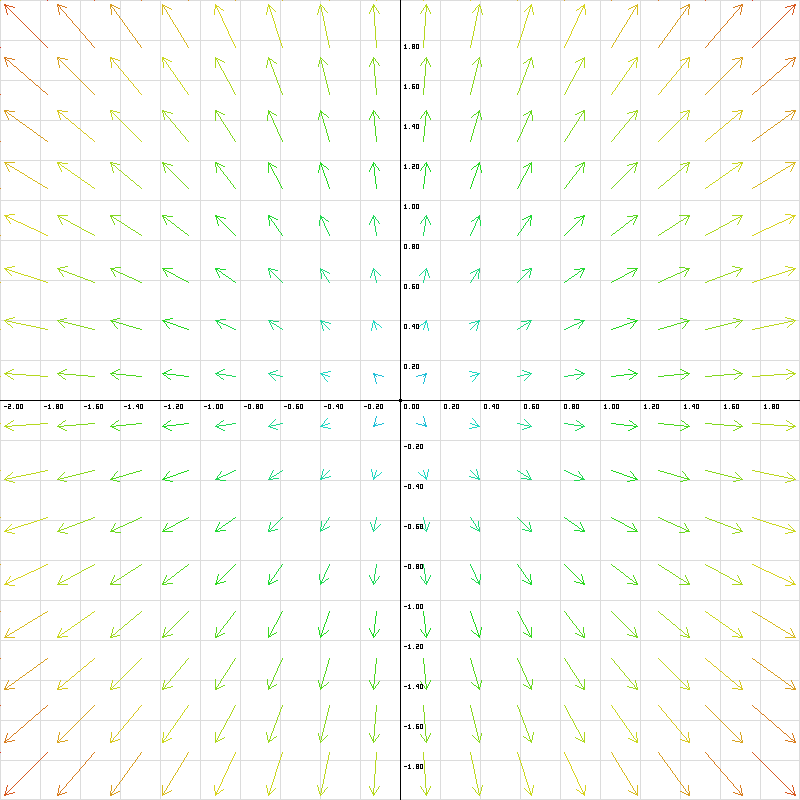
\includegraphics[scale=0.45]{x2y2.png}
	\centering
	\caption{Vector field for $f(x,y)=\begin{bmatrix}2x\\2y\end{bmatrix}$}
	\label{fig:x2y2}
\end{figure}

The nabla operator proves foundational to several important concepts within vector calculus, as will be demonstrated.

\subsubsection*{Directional derivatives}
Partial derivatives allow for the computation of derivatives in the $x$ and $y$, and this concept may be extended to the derivative in any direction $\vec{v}$. Since $\nabla f$ computes the rate of change in the $x$ and $y$ directions, dotting this vector with some directional vector $\vec{v}$ gives the directional derivative in the direction of $\vec{v}$, denoted as:
\begin{equation}
	\nabla_{\vec{v}}f=\nabla f\cdot\vec{v}
\end{equation}
Nabla pointing in the direction of greatest ascent can be proven using the directional derivative.
\begin{proof}\label{p:nablagreatestchange}
	\begin{align*}
		\nabla_{\vec{v}}f&=\nabla f\cdot\vec{v}\\
		\max\nabla_{\vec{v}}f&\rightarrow\text{direction of greatest change}\\
		\max\nabla_{\vec{v}}f&=\max\nabla f\cdot\vec{v}\\
		&=\max\lVert\nabla f\rVert\lVert\vec{v}\rVert\cos{\theta}\\
		&\leadsto\theta=0\\
		&\implies\max\nabla_{\vec{v}}f\text{ points in the direction of }\nabla f
	\end{align*}
\end{proof}
\subsubsection*{Other}
$$f:\mathbb{R}^n\rightarrow\mathbb{R}^n\ni n>1,n\in\mathbb{Z}$$
\begin{equation}
	\materialder{f}{t}\definedas\partialder{f}{t}+\underbrace{\vec{v}\cdot\nabla f}_{\hidewidth\text{Directional derivative }\nabla_{\vec{v}}f\hidewidth}
\end{equation}
$$\vec{v_1}\otimes\vec{v_2}$$

% > fluid dynamics
\subsection{Incompressible flow}
An incompressible fluid is any fluid such that $\divergence\fatf=0$, which is to say that the divergence of the fluid is 0.

\subsection{Complex analysis in 2D potential flow}

% > the navier-stokes equations
\subsection*{Green's theorem}\label{sec:greenstheorem}
\begin{equation} % navier-stokes
	\materialder{f}{\mathbf{t}}=\iiint\limits_{V}(\materialder{\rho}{\mathbf{t}}+\rho(\nabla\cdot u))dV
\end{equation}
Lorem ipsum dolor sit amet \cite{peyret2012computational}

\section{Modeling flow around circular obstacles}
\subsection{Ideal potential flow model}
\subsection{Effect of circulation on flow patterns}
\section{Real-world observations}
\section{Results}
\section{Conclusion}
\newpage
\bibliographystyle{apalike}
\bibliography{sources}
\stepcounter{section}
\addcontentsline{toc}{section}{\protect\numberline{\thesection}List of Figures}
\renewcommand{\listfigurename}{\thesection\hspace{20pt}List of Figures}\listoffigures
\newpage
\section{Research}
\subsection{Potential flow around a circular cylinder}
A cylinder of radius $L$ is placed in two-dimensional, incompressible, inviscid flow which flows in the direction of $\ihat$.
Far away from the cylinder the velocity field $\mathbf{V}$ can be described as: 
\begin{equation}\label{equation:in-infinitum}
	\mathbf{V}=U\ihat
\end{equation}
Where $U$ is some constant. Since the cylinder is impermissible, at the boundary $\mathbf{V}\cdot\nhat=0$ where the vector $\nhat$ is the unit vector normal to the surface. 

Since in this model the viscosity $\nu=0$, the flow can be modelled using the Euler equations. If the Euler equations, apply, so does Kelvin's theorem:
\begin{theorem}[Kelvin's circulation theorem]\label{theorem:kelvin}
	The circulation around a closed material loop moving with an inviscid, barotropic fluid in the presence of conservative body forces remains constant over time.\needcitation
	
	If $\Gamma$ denotes the circulation around a material loop $C(t)$ moving with the fluid, then:
	$$\materialder{\Gamma}{t}=0$$
\end{theorem}

\textit{Id est}, if the vorticity of $\mathbf{V}$ is $0$ initially, it must remain $0$ everywhere, thus $\curl\mathbf{V}=0$. Since the flow is irrotational, $\mathbf{V}$ can be expressed as $\mathbf{V}=\nabla\phi$, where $\phi$ is the velocity potential.

Furthermore, if $\mathbf{V}$ is incompressible, that being that $\divergence\mathbf{V}=0$, then $\phi$ must satisfy Laplace's equation: $\laplacian{\phi}=0$.

\subsection{Polar coordinate boundary conditions}
\subsubsection{$\mathbf{V}=U\ihat$}\label{sec:vuihat}
In polar coordinates, the base vectors $\rhat$ and $\thetahat$ are defined as:
\begin{align*}
	\rhat&\definedas\ihat\cos\theta+\jhat\sin\theta\\
	\thetahat&\definedas-\ihat\sin\theta+\jhat\cos\theta
\end{align*}
Solving for $\ihat$ and $\jhat$ gives:
\begin{align}
	\label{poihat:1}\ihat&=\frac{\rhat-\jhat\sin\theta}{\cos\theta}\\
	\label{poihat:2}\jhat&=\frac{\thetahat+\ihat\sin\theta}{\cos\theta}
\end{align}
Substituting \ref{poihat:2} into \ref{poihat:1} and isolating $\ihat$ shows that
\begin{align}
	\notag\ihat&=\frac{\rhat-\frac{\thetahat+\ihat\sin\theta}{\cos\theta}\sin\theta}{\cos\theta}\\
	\notag&=\frac{\rhat}{\cos\theta}-\frac{\thetahat\sin\theta+\ihat\sin^2\theta}{\cos^2\theta}\\
	\notag&=\frac{\rhat}{\cos\theta}-\frac{\thetahat\sin\theta}{\cos^2\theta}-\frac{\ihat\sin^2\theta}{\cos^2\theta}\\
	\notag\implies\ihat+\frac{\sin^2\theta}{\cos^2\theta}\ihat&=\frac{\rhat}{\cos\theta}-\frac{\thetahat\sin\theta}{\cos^2\theta}\\
	\notag\ihat\left(1+\frac{\sin^2\theta}{\cos^2\theta}\right)&=\frac{\rhat}{\cos\theta}-\frac{\thetahat \sin\theta}{\cos^2\theta}\\
	\notag\ihat\left(\frac{\sin^2\theta+\cos^2\theta}{\cos^2\theta}\right)&=\frac{\rhat}{\cos\theta}-\frac{\thetahat \sin\theta}{\cos^2\theta}\\
	\notag\frac{\ihat}{\cos^2\theta}&=\frac{\rhat}{\cos\theta}-\frac{\thetahat \sin\theta}{\cos^2\theta}\\
	\label{poihat:3}\ihat&=\rhat\cos\theta-\thetahat\sin\theta\qed
\end{align}
The condition stated in \ref{equation:in-infinitum} was that \textit{in infinitum}, $\mathbf{V}=U\ihat$\,. By substituting in \ref{poihat:3}, the statement becomes in terms of $\rhat$ and $\thetahat$:
$$
	\mathbf{V}=U(\rhat\cos\theta-\thetahat\sin\theta)\quad\text{as}\quad r\rightarrow\infty
$$

\subsubsection{$\mathbf{V}\cdot\nhat=0$}\label{sec:vdotnhatzero}
In polar coordinates, the base vector $\rhat$ points in the direction of positive change of $r$, that being outwards from the center. If the cylinder is assumed to be the center of the coordinate system, then $\rhat$ will always point normal to the surface of the cylinder. Therefore, at the boundary of the cylinder when $r=L$,
$$\begin{matrix}
	\mathbf{V}\cdot\rhat=0
\end{matrix}$$

\subsubsection{$\laplacian{\phi}=0$}\label{sec:deltaphizero}
% Come up with a better name later
\begin{lemma}[Jacobian Shmaycobian]
	The derivative of composite functions corresponds to the product Jacobian of Jacobian matrices:
	$$J_{f\circ g}=(J_f\circ g)J_g$$
\end{lemma}
\begin{proof}
	I finna fix it later frfr.
\end{proof}

\begin{lemma}[Multivariable chain rule]
Let $X(t,u)$ and $Y(t,u)$ be functions where $X,Y:\mathbb{R}^2\rightarrow\mathbb{R}$ such that $X,Y\in C^1(\mathbb{R}^2)$. Then define $Z(x,y)$ to be a function where $Z:\mathbb{R}^2\rightarrow\mathbb{R}$ and $Z\in C^1(\mathbb{R}^2)$. Then the partial derivatives of the composite function $z(t,u)=Z(X(t,u),Y(t,u))$ are given by:
\begin{align*}
	\pdv{z}{t}&=\pdv{Z}{x}\pdv{X}{t}+\pdv{Z}{y}\pdv{Y}{t}\\
	\pdv{z}{u}&=\pdv{Z}{x}\pdv{X}{u}+\pdv{Z}{y}\pdv{Y}{u}
\end{align*}
\begin{proof}
	Let $g:\mathbb{R}^n\rightarrow\mathbb{R}^p$ and $f:\mathbb{R}^p\rightarrow\mathbb{R}^m$, the dimensions of the Jacobian matrices must then be given as:
	\begin{gather*}
		J_g\in\mathbb{R}^{m\times p},\,(J_f\circ g)\in\mathbb{R}^{p\times n}\\
		\therefore(J_f\circ g)J_g\in\mathbb{R}^{n\times m}
	\end{gather*}
	Let the parameters of $f$ be called $x_1,\,x_2,\,\hdots,\,x_n$ and the parameters of $g$ be called $y_1,\,y_2,\,\hdots,\,y_n$. The Jacobian of the the composite function $f\circ g$ is defined as:
	\begin{gather*}
		J_{f\circ g}=\begin{bmatrix}
			\pdv{f}{y_1}&\pdv{f}{y_2}&\hdots&\pdv{f}{y_n}
		\end{bmatrix}.
	\end{gather*}
	Because $f\circ g:\mathbb{R}^n\rightarrow\mathbb{R}^m$, $J_{f\circ g}\in\mathbb{R}^{n\times m}$. The element at position $(i,j)$ of some Jacobian $J_F$ is given by:
	\begin{equation}
		\label{chainrule:1}(J_F)_{ij}=\pdv{(f\circ g)_j}{x_i}\\
	\end{equation}
	% (\mathbf{A}\mathbf{B})_{ij}=\sum_{k=1}^pa_{ik}b_{kj}\\
	By matrix multiplication, $((J_f\circ g)J_g)_{ij}$ can be computed as:
	$$
		\left((J_f\circ g)J_g\right)_{ij}=\sum_{k=1}^p(J_f\circ g)_{ik}(J_g)_{kj}
	$$
	Applying the form given in \ref{chainrule:1} gives:
	\begin{align}
		\notag\left((J_f\circ g)J_g\right)_{ij}&=\sum_{k=1}^p\eval{\pdv{f_k}{x_i}}_{x=g}\pdv{g_j}{y_k}\\
		\leadsto\left((J_f\circ g)J_g\right)_{ij}&=\sum_{k=1}^p\pdv{f}{g}\pdv{g}{y_k}\qedhere
	\end{align}
	For the case given above with the composite function $z$,
	\begin{align*}
		J_z=
	\end{align*}
\end{proof}
\end{lemma}

\begin{lemma}[Polar-Form Laplacian]
	For some scalar field $\phi(x,y)$ defined in a Cartesian system, the Laplacian of $\phi$ in polar coordinates $\langle r,\theta\rangle$ is given by:
	$$
	\laplacian{\phi}=\pdv[2]{\phi}{r}+\frac{1}{r}\pdv{\phi}{r}+\frac{1}{r^2}\pdv[2]{\phi}{\theta}
	$$
\end{lemma}
\begin{proof}
	In Cartesian coordinates, the Laplacian operator $\laplacian$ is defined as $\nabla\cdot\nabla$, which for the scalar field $\phi$ becomes:
	\begin{align*}
		\notag\laplacian{\phi}&=\div\nabla\phi\\
							  &=\begin{pmatrix}\pdv*{x}\\\pdv*{y}\end{pmatrix}\vdot\begin{pmatrix}\pdv*{\phi}{x}\\\pdv*{\phi}{y}\end{pmatrix}\\
							  &=\pdv[2]{\phi}{x}+\pdv[2]{\phi}{y}
	\end{align*}
	Translating $x$ and $y$ to polar coordinates and calculating their derivatives with respect to $r$ and $\theta$ gives:
	\begin{align}
		\notag x=r\cos\theta&,\quad y=r\sin\theta\\
		\label{polap:1}\pdv{x}{r}=\cos\theta&,\quad\pdv{y}{r}=\sin\theta\\
		\label{polap:2}\pdv{x}{\theta}=-r\sin\theta&,\quad\pdv{y}{\theta}=r\cos\theta
	\end{align}
	Consequently, by the chain rule and substitution from \ref{polap:1}:
	\begin{align}
		\notag\pdv{\phi}{r}&=\pdv{\phi}{x}\pdv{x}{r}+\pdv{\phi}{y}\pdv{y}{r}\\
		\label{polap:3}&=\pdv{\phi}{x}\cos\theta+\pdv{\phi}{y}\sin\theta
	\end{align}
	Taking the derivative of \ref{polap:3} with respect to $r$ again gives:
	\begin{align}
		\notag\pdv[2]{\phi}{r}&=\pdv{}{r}\pdv{\phi}{x}\cos\theta+\pdv{}{r}\pdv{\phi}{y}\sin\theta\\
		\label{polap:4}&=\pdv{}{x}\pdv{\phi}{r}\cos\theta+\pdv{}{y}\pdv{\phi}{r}\sin\theta
	\end{align}
	Substituting \ref{polap:3} into \ref{polap:4} gives:
	\begin{align}
		\notag\pdv[2]{\phi}{r}&=\pdv{}{x}\left(\pdv{\phi}{x}\cos\theta+\pdv{\phi}{y}\sin\theta\right)\cos\theta+\pdv{}{y}\left(\pdv{\phi}{x}\cos\theta+\pdv{\phi}{y}\sin\theta\right)\sin\theta\\
		\notag&=\pdv[2]{\phi}{x}\cos^2\theta+\pdv{\phi}{x}{y}\sin\theta\cos\theta+\pdv{\phi}{y}{x}\cos\theta\sin\theta+\pdv[2]{\phi}{y}\sin^2\theta\\
		\label{polap:5}&=\pdv[2]{\phi}{x}\cos^2\theta+2\pdv{\phi}{x}{y}\sin\theta\cos\theta+\pdv[2]{\phi}{y}\sin^2\theta
	\end{align}
	Applying the same process for $\pdv{\phi}{\theta}$ with substitution from \ref{polap:2} yields:
	\begin{align}
		\notag\pdv{\phi}{\theta}&=\pdv{\phi}{x}\pdv{x}{\theta}+\pdv{\phi}{y}\pdv{y}{\theta}\\
		\label{polap:6}&=-\pdv{\phi}{x}r\sin\theta+\pdv{\phi}{y}r\cos\theta
	\end{align}
	Taking the derivative of \ref{polap:6} with respect to $\theta$ again gives:
	\begin{align}
		\notag\pdv[2]{\phi}{\theta}&=-\pdv{}{\theta}\pdv{\phi}{x}r\sin\theta+\pdv{}{\theta}\pdv{\phi}{y}r\cos\theta
	\end{align}
	Since both terms contain a product of two functions dependent on $\theta$ the product rule needs to be applied. This gives:
	\begin{align}
		\notag\pdv[2]{\phi}{\theta}&=-\pdv{\phi}{\theta}{x}r\sin\theta-\pdv{\phi}{x}r\cos\theta+\pdv{\phi}{\theta}{y}r\cos\theta-\pdv{\phi}{y}r\sin\theta\\
		\label{polap:7}&=-r\left(\pdv{\phi}{x}\cos\theta+\pdv{\phi}{y}\sin\theta\right)+r\pdv{\phi}{\theta}\left(-\pdv{}{x}\sin\theta+\pdv{}{y}\cos\theta\right)
	\end{align}
	Substituting \ref{polap:6} into \ref{polap:7} gives:
	\begin{align}
		\label{polap:8}\pdv[2]{\phi}{\theta}&=-r\left(\pdv{\phi}{x}\cos\theta+\pdv{\phi}{y}\sin\theta\right)+r\underbrace{\left(-\pdv{\phi}{x}r\sin\theta+\pdv{\phi}{y}r\cos\theta\right)\left(-\pdv{}{x}\sin\theta+\pdv{}{y}\cos\theta\right)}_{\Phi}
	\end{align}
	Expanding $\Phi$:
	\begin{align}
		\notag\Phi&=\left(-\pdv{\phi}{x}r\sin\theta+\pdv{\phi}{y}r\cos\theta\right)\left(-\pdv{}{x}\sin\theta+\pdv{}{y}\cos\theta\right)\\
		\notag&=\left(-\pdv{\phi}{x}r\sin\theta\right)\left(-\pdv{}{x}\sin\theta\right)+\left(-\pdv{\phi}{x}r\sin\theta\right)\left(\pdv{}{y}\cos\theta\right)\\
		\notag&+\left(\pdv{\phi}{y}r\cos\theta\right)\left(-\pdv{}{x}\sin\theta\right)+\left(\pdv{\phi}{y}r\cos\theta\right)\left(\pdv{}{y}\cos\theta\right)\\
		\notag&=\pdv[2]{\phi}{x}r\sin^2\theta-2\pdv{\phi}{x}{y}r\cos\theta\sin\theta+\pdv[2]{\phi}{y}r\cos^2\theta
	\end{align}
	Substituting $\Phi$ back into \ref{polap:8} gives:
	\begin{align}
		\notag\pdv[2]{\phi}{\theta}&=-r\left(\pdv{\phi}{x}\cos\theta+\pdv{\phi}{y}\sin\theta\right)+r\left(\pdv[2]{\phi}{x}r\sin^2\theta-2\pdv{\phi}{x}{y}r\cos\theta\sin\theta+\pdv[2]{\phi}{y}r\cos^2\theta\right)\\
		\notag&=r^2\left(\pdv[2]{\phi}{x}\sin^2\theta-2\pdv{\phi}{x}{y}\cos\theta\sin\theta+\pdv[2]{\phi}{y}\cos^2\theta\right)-r\left(\pdv{\phi}{x}\cos\theta+\pdv{\phi}{y}\sin\theta\right)\\
		\label{polap:9}&=r^2\left(\pdv[2]{\phi}{x}\sin^2\theta-2\pdv{\phi}{x}{y}\cos\theta\sin\theta+\pdv[2]{\phi}{y}\cos^2\theta\right)-r\pdv{\phi}{r}
	\end{align}
	Combining \ref{polap:5} and \ref{polap:9} yields:
	\begin{align}
		\notag\pdv[2]{\phi}{r}+\pdv[2]{\phi}{\theta}&=\pdv[2]{\phi}{x}\cos^2\theta+2\pdv{\phi}{x}{y}\sin\theta\cos\theta+\pdv[2]{\phi}{y}\sin^2\theta\\
		\notag&+r^2\left(\pdv[2]{\phi}{x}\sin^2\theta-2\pdv{\phi}{x}{y}\cos\theta\sin\theta+\pdv[2]{\phi}{y}\cos^2\theta\right)-r\pdv{\phi}{r}\\
		\notag\implies\notag\pdv[2]{\phi}{r}+\frac{1}{r^2}\pdv[2]{\phi}{\theta}&=\pdv[2]{\phi}{x}\cos^2\theta+\pdv[2]{\phi}{x}\sin^2\theta+\pdv[2]{\phi}{y}\cos^2\theta+\pdv[2]{\phi}{y}\sin^2\theta-\frac{1}{r}\pdv{\phi}{r}\\
		\notag&=\pdv[2]{\phi}{x}\left(\cos^2\theta+\sin^2\theta\right)+\pdv[2]{\phi}{y}\left(\cos^2\theta+\sin^2\theta\right)-\frac{1}{r}\pdv{\phi}{r}\\
		\notag&=\pdv[2]{\phi}{x}+\pdv[2]{\phi}{y}-\frac{1}{r}\pdv{\phi}{r}\\
		\notag\implies\pdv[2]{\phi}{x}+\pdv[2]{\phi}{y}&=\pdv[2]{\phi}{r}+\frac{1}{r}\pdv{\phi}{r}+\frac{1}{r^2}\pdv[2]{\phi}{\theta}\\
		\label{polap:final}\therefore\laplacian{\phi}&=\pdv[2]{\phi}{r}+\frac{1}{r}\pdv{\phi}{r}+\frac{1}{r^2}\pdv[2]{\phi}{\theta}
	\end{align}	
\end{proof}

\subsection{Ad confluōrem}
Summarized, the conditions translated to polar form in sections \ref{sec:vuihat}, \ref{sec:vdotnhatzero} and \ref{sec:deltaphizero} are:
$$\begin{matrix}
	&\mathbf{V}=U(\rhat\cos\theta-\thetahat\sin\theta)\quad&\text{as}\quad&r\rightarrow\infty\vecpadding\\
	&\mathbf{V}\cdot\rhat=0\quad&\text{when}\quad&r=L\vecpadding\\
	&\dfrac{\partial^2\phi}{\partial r^2}+\dfrac{1}{r}\dfrac{\partial\phi}{\partial r}+\dfrac{1}{r^2}\dfrac{\partial^2\phi}{\partial\theta^2}=0
\end{matrix}$$

testing hello hello!\cite{mat132-episode25}

\end{document}